\begin{figure}[tbp]
\centering
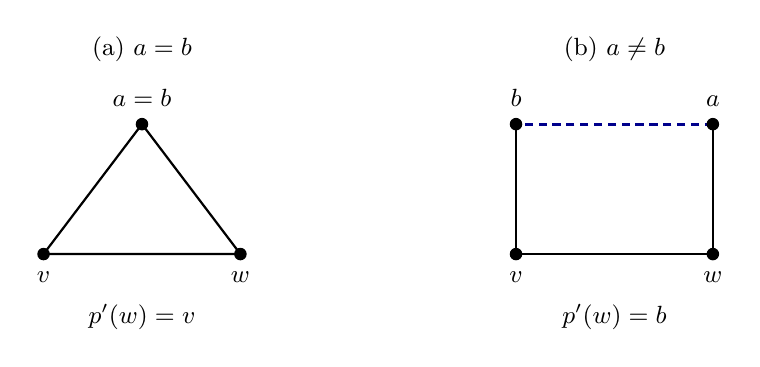
\begin{tikzpicture}[
  x=1cm,y=1cm,font=\small,
  vertex/.style={circle,fill=black,inner sep=1.6pt},
  every path/.style={line width=.8pt}
]
\node at (1.25,2.6) {(a) $a=b$};
\node at (7.25,2.6) {(b) $a\ne b$};
\draw (0,0)--(2.5,0)--(1.25,1.65)--cycle;
\node[vertex,label=below:$v$] at (0,0) {};
\node[vertex,label=below:$w$] at (2.5,0) {};
\node[vertex,label=above:{$a=b$}] at (1.25,1.65) {};
\node at (1.25,-.8) {$p'(w)=v$};
\draw (6,1.65)--(6,0)--(8.5,0)--(8.5,1.65);
\draw[blue!55!black,densely dashed,line width=1pt] (8.5,1.65)--(6,1.65);
\node[vertex,label=below:$v$] at (6,0) {};
\node[vertex,label=below:$w$] at (8.5,0) {};
\node[vertex,label=above:$b$] at (6,1.65) {};
\node[vertex,label=above:$a$] at (8.5,1.65) {};
\node at (7.25,-.8) {$p'(w)=b$};
\end{tikzpicture}
\caption{The two partner updates in the link of
$D=S\setminus\{v,w\}$. Put $a=p(v)$ and $b=p(w)$, and replace
$v$ by $a$ in the tetrahedron $S$. The new partner map is $p'$.
The known edges $\{v,w\}$, $\{w,a\}$ and $\{v,b\}$ form a triangle
when $a=b$. When $a\ne b$, they form a path on four vertices; the
short-link condition forces the closing edge $\{a,b\}$ (dashed).
In both cases $p'(a)=v$, and the blocks retain their elements.}
\label{fig:partner-links}
\end{figure}
